% This file was created with tikzplotlib v0.10.1.
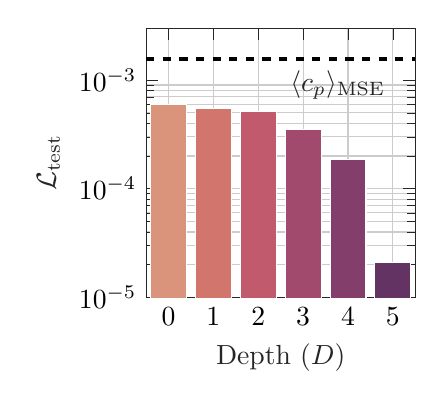
\begin{tikzpicture}

\definecolor{darksalmon217148123}{RGB}{217,148,123}
\definecolor{darkslateblue9951100}{RGB}{99,51,100}
\definecolor{darkslategray38}{RGB}{38,38,38}
\definecolor{darkslategray66}{RGB}{66,66,66}
\definecolor{dimgray13162108}{RGB}{131,62,108}
\definecolor{indianred16174110}{RGB}{161,74,110}
\definecolor{indianred19290108}{RGB}{192,90,108}
\definecolor{indianred209117109}{RGB}{209,117,109}
\definecolor{lightgray204}{RGB}{204,204,204}

\begin{axis}[
width=5cm,
height=5cm,
axis line style={darkslategray38},
log basis y={10},
tick align=inside,
unbounded coords=jump,
x grid style={lightgray204},
xlabel=\textcolor{darkslategray38}{Depth (\(\displaystyle D\))},
xmajorticks=true,
xmin=-0.5, xmax=5.5,
xminorgrids,
xmajorgrids,
xtick style={color=darkslategray38},
xtick={0,1,2,3,4,5},
xticklabels={
  \(\displaystyle {0}\),
  \(\displaystyle {1}\),
  \(\displaystyle {2}\),
  \(\displaystyle {3}\),
  \(\displaystyle {4}\),
  \(\displaystyle {5}\)
},
y grid style={lightgray204},
ylabel=\textcolor{darkslategray38}{\(\displaystyle \mathcal{L}_{\mathrm{test}}\)},
ymajorticks=true,
ymin=1e-5, ymax=0.003,
yminorgrids,
ymode=log,
ytick style={color=darkslategray38},
]

\def\epsVal{1e-8}

\draw[draw=white,fill=darksalmon217148123] (axis cs:-0.4,\epsVal) rectangle (axis cs:0.4,0.000597328355);
\draw[draw=white,fill=indianred209117109] (axis cs:0.6,\epsVal) rectangle (axis cs:1.4,0.000545040821);
\draw[draw=white,fill=indianred19290108] (axis cs:1.6,\epsVal) rectangle (axis cs:2.4,0.000514299027);
\draw[draw=white,fill=indianred16174110] (axis cs:2.6,\epsVal) rectangle (axis cs:3.4,0.000353918178);
\draw[draw=white,fill=dimgray13162108] (axis cs:3.6,\epsVal) rectangle (axis cs:4.4,0.000186683203);
\draw[draw=white,fill=darkslateblue9951100] (axis cs:4.6,\epsVal) rectangle (axis cs:5.4,2.07822668e-05);
\addplot [line width = 1.5pt, dashed, black]
table {%
-0.5 0.0015630356362404
5.5 0.0015630356362404
};
\addplot [line width=1.08pt, darkslategray66]
table {%
0 nan
0 nan
};
\addplot [line width=1.08pt, darkslategray66]
table {%
1 nan
1 nan
};
\addplot [line width=1.08pt, darkslategray66]
table {%
2 nan
2 nan
};
\addplot [line width=1.08pt, darkslategray66]
table {%
3 nan
3 nan
};
\addplot [line width=1.08pt, darkslategray66]
table {%
4 nan
4 nan
};
\addplot [line width=1.08pt, darkslategray66]
table {%
5 nan
5 nan
};

\draw (axis cs:2.5,0.0009) node[
  scale=1,
  anchor=west,
  text=darkslategray38,
  rotate=0.0
]{$ \langle c_p \rangle _ {\mathrm{MSE}}$};
\end{axis}

\end{tikzpicture}
